\section{Sicherheitsaspekte}\label{s:Sicherheitsaspekte}

Über das Internet werden  immer mehr Informationen versendet. Ein kleiner Bestandteil hiervon sind auch die Informationen die verschiedene Geräte des \ac{IoT}s untereinander austauschen.
Diese automatisch abgewickelte \ac{M2M}-Kommunikation stellt ein hohes Sicherheitsrisiko für Unternehmen und Privatpersonen dar. Durch einen gezielten Angriff könnten personenbezogene oder sicherheitsrelevante Informationen an die Öffentlichkeit gelangen. Aufgrund dessen müssen sich die Verantwortlichen die Frage stellen, wie man mit dieser Herausforderung in der Zukunft umgeht. 

Sicherheitsexperten sind sich bereits heute einig, dass das \ac{IoT} ein enormes Risiko darstellt\cite{ws:iotsec}. Für Privatpersonen äußert sich das hauptsächlich in der Sicherheit ihrer Elektronischen Geräte. So musste der Automobilhersteller BMW kürzlich ein Softwareupdate für seine Automobile mit dem ConnectedDrive-System ausliefern, da es Hackern ohne Spuren zu hinterlassen gelungen war, die Türen mittels Smartphones zu öffnen \cite{ws:zeitbmw}.\\

Zusätzlich zur Beschädigung oder Entwendung von Eigentum durch Hacker besteht ein Risiko private Informationen zu verlieren. Gerade Informationen wie E-Mail-Adressen oder Passwörter stehen in großem Interesse der Hacker. Solche könnten über ein privates \ac{IoT} entwendet werden und für weitere Cyber-Kriminelle Aktionen genutzt werden. \\

Auch Firmen müssen sich die Risiken bewusst machen, die sie durch die Benutzung von \ac{IoT}-Geräten eingehen. Oftmals nutzen Unternehmen \ac{IoT}-Systeme als Infrastrukturkomponenten über die sie einen Service betreiben. Solche Netze stellen einen Idealen Angriffspunkt für Wirtschaftsspionage oder Denial of Service - Attacken dar. Bricht ein Hacker in solche Systeme ein, wird es ihm schnell möglich sein einen Millionenschaden anzurichten.


Da die Entwicklung des \ac{IoT} derzeit noch an fahrt aufnimmt, muss jedem Nutzer bewusst sein, dass auch die Sicherheit noch nicht vollständig Entwickelt ist. Viele Aspekte werden sich in den nächsten Jahren weiterentwickeln, die Sicherheit wird jedoch zunehmend eine der wichtigsten Komponenten des \ac{IoT}s.\\


Jede am \ac{IoT} teilnehmende Komponente muss einen Zugang zur aufgebauten Netzwerkumgebung besitzen um ihre Metadaten an andere Teilnehmer zu kommunizieren. Über diese zusammengesammelten Informationen trifft das System eine Entscheidung zu handeln. Hierbei entsteht ein Sicherheitsrisiko.\\
Mit netzwerkfähigen Geräten ist es möglich, sich in das aufgebaute Netzwerk einzuklinken, und sich ebenfalls als Komponente auszugeben. Dies ermöglicht einem Angreifer Daten abzufangen oder zu seinen Zwecken zu manipulieren. Dies kann das verhalten des Gesamten Systems verändern.\\
Ebenfalls ist es möglich, dass ein Angreifer ein Teilnehmer des \ac{IoT}s übernimmt und somit Zugriff auf das Netzwerk erhält.\\

\subsection{Sicherheitsmodell nach Gordon Cooper}\label{ss:Sicherheitsmodell}


Wie schützt man das \ac{IoT}?\\

Um diese Frage beantworten zu können müssen die Schnittstellen Eckpunkte des \ac{IoT}s definiert werden die Hackern Angriffsflächen bieten. Zu diesem Zweck hat Gordon Cooper ein Sicherheitsmodell aufgestellt, anhand dessen Sicherheitsmaßnahmen erklärt werden können. Dieses Sicherheitsmodell wird im Abbildung ~\ref{f:security} dargestellt.

\vspace{5 mm}
\begin{figure}[H] 
	\centering
	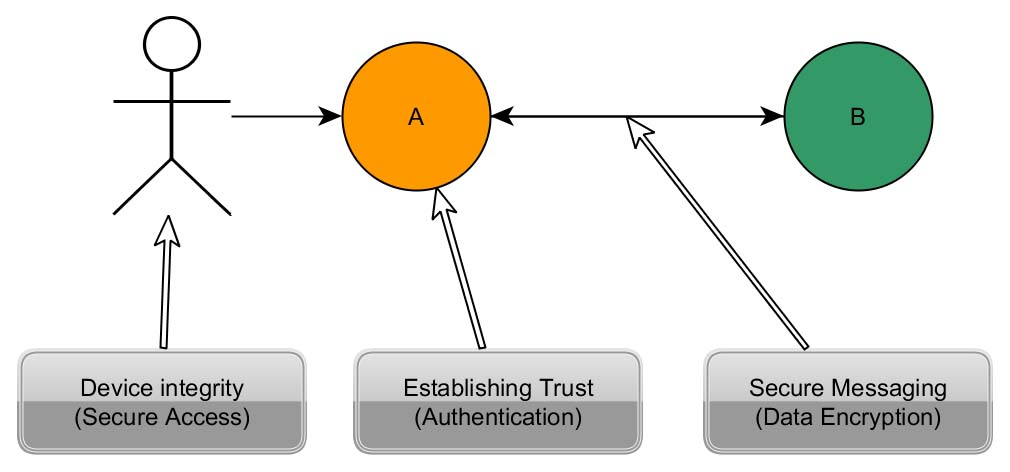
\includegraphics[scale=0.4]{Bilder/sicherheitsmodell}
	\caption{Sicherheitsmodell nach Gordon Cooper\cite{z:DesignElektronik}}
	\label{f:security}
\end{figure}
\vspace{5 mm}

Um die Integrität der \ac{IoT}-Komponenten zu schützen muss der Zugang und somit die Anmeldung an jedem Knoten geschützt werden. Dies wird im Sicherheitsmodell nach Gordon Cooper als "Secure Access" bezeichnet.\\
Wie im privaten wird auch das Funknetz in dem sich die Teilnehmer des \ac{IoT}s einklinken durch einen Sicherheitsschlüssel geschützt. Dieser muss von den Geräten, sowie allen Benutzern angegeben werden um Zugang zum Netz zu erhalten. Eine wichtige Aufgabe besteht darin diesen Schlüssel zu schützen. Hierbei muss unter anderem die Weitergabe sowie die Kommunikation im Netz durchdacht und überwacht werden. Besonders bei der Schlüsselwahl ist Vorsicht geboten. Es sollten niemals Namen, Geburtsdaten oder andere Informationen die einer Person zugeordnet werden können verwendet werden. Zusätzlich sind gebräuchliche Wörter nicht empfehlenswert, da diese leicht durch Wörterbuchangriffe überlistet werden können. Damit die Sicherheit des Passworts gewährleistet, sollte es mindestens 8 Zeichen enthalten und groß/klein Schreibung, sowie Sonderzeichen und Zahlen enthalten. Eine allgemeingültige Faustregel ist: Umso Länger, Umso besser.\\

Eine weitere Sicherheitsmaßnahme sind maßgeschneiderte Zugriffsrechte. Jeder Teilnehmer im \ac{IoT} darf nur so viele Rechte besitzen, wie unbedingt nötig. Hierdurch wird sichergestellt, dass Angreifer beim Erlangen eines Zugangscodes nur eingeschränkte Handlungsmöglichkeiten besitzen und der möglicher Schaden gering gehalten wird.\\

Um die Anmeldung an \ac{IoT}-Geräten möglichst Sicher zu gestalten sollte ein asymmetrisches Schlüsselpaar verwendet werden. Hierbei wird pro Kommunikationsteilnehmer ein Schlüsselpaar verwendet, das aus einem öffentlichen Schlüssel, dem "Public Key" und einem privaten Schlüssel, dem "Private Key" besteht. Wie der Name bereits sagt, ist der "Private Key" nur beim Schlüsselinhaber vorzufinden und darf nicht öffentlich werden. Der "Public Key" hingegen wird jedem Kommunikationspartner bereitgestellt und kann über unsichere Kommunikationswege geteilt werden.\\

Die Verschlüsselung der Kommunikation geschieht mit einem Algorithmus, der das Entschlüsseln nur mit dem nicht zum Verschlüsseln verwendeten Schlüssel ermöglicht. Dies bedeutet, dass von dem Inhaber des "Private Keys" versendete Nachrichten auch unbestreitbar von ihm stammen. Durch die hiermit stattfindende Authentifikation wird der zweite Sektor "Authentication" des Sicherheitsmodells nach Gordon Cooper erfüllt.\\

Da jede Kommunikation zwischen zwei \ac{IoT}-Komponenten potentiell sensible Daten beinhalten kann, muss permanent ein verschlüsselter Kanal verwendet werden. Dies ist im Sicherheitsmodell mit dem Sektor "'Secure Messaging - Data Encryption" beschrieben. Um dies performant zu gestalten wird das beschriebene Public-Key-Verfahren genutzt, um einen symmetrischen Schlüssel auszuhandeln. Bei diesem handelt es sich um einen Schlüssel, der sowohl zum Ver- als auch Entschlüsseln verwendet wird. Dieser Session-Key genannte Sitzungsschlüssel wird bei der Kommunikationsaufnahme der Komponenten generiert und mithilfe des Public-Keys des Kommunikationspartners verschlüsselt. Daraufhin ist es dem Empfänger möglich den symmetrischen Schlüssel für die weitere Kommunikation zu verwenden. Da der Session-Key bei jeder Sitzung neu ausgehandelt wird, ist er nur den Kommunikationspartnern bekannt und bietet ausreichende Sicherheit.\\
\subsection{Verschlüsselungsstandard AES}\label{ss:AES}

Der aktuell gültige Kryptographiestandard ist der im Jahr 2000 veröffentlichte \ac{AES}. Bei diesem Verfahren wird eine symmetrische Block-Cipher verwendet, die mit einem 128, 192 oder 256 Bits langen Schlüssel gleichlange Datenblöcke verschlüsselt\cite{ws:AES}.\\
Solange ein Verschlüsselungsverfahren wie \ac{AES} nicht durchbrochen wird, kann es nur durch sogenannte Brute-Force-Attacken angegriffen werden. Hierbei werden alle Möglichkeiten durchprobiert, bis man zufällig auf den richtigen Schlüssel trifft. Bei \ac{AES} mit 128 Bit Schlüssellänge sind hierfür bis zu $2^{128}\equiv 3,4*10^{38}$ Versuche nötig. Bei 256 Bit sind es bereits $2^{256}\equiv 1.2*10^{77}$ Versuche. Selbst mit Hilfe der aktuellsten Supercomputer würde dies Millionen Jahre in Anspruch nehmen.\\

\begin{table}[H] 
	\centering
	\begin{tabular}{|c|c|}\hline
		Schlüssellänge & Kombinationsmöglichkeiten\\ \hline \hline
		1-Bit & 2 \\ \hline
		2-Bit & 4 \\ \hline
		4-Bit & 16 \\ \hline
		8-Bit & 256 \\ \hline
		16-Bit & 65536 \\ \hline
		32-Bit & 4.2*10\textsuperscript{9} \\ \hline
		56-Bit (DES) & 7.2*10\textsuperscript{16} \\ \hline
		64-Bit  & 1.8*10\textsuperscript{19} \\ \hline
		128-Bit(AES) & 3.4*10\textsuperscript{38} \\ \hline
		192-Bit(AES) & 6.2*10\textsuperscript{57} \\ \hline
		256-Bit (AES) &  1.2*10\textsuperscript{77} \\ \hline
	\end{tabular}
	\caption{Kombinationsmöglichkeiten bei verschiedenen Schlüssellängen}
	\label{t:keylength}
\end{table}
\vspace{5 mm}

Jede in \ac{AES} erlaubte Schlüssellänge bietet aufgrund des komplexen Verschlüsselungsverfahrens und der daraus resultierenden Rechenzeit pro Angriff ausreichende Sicherheit. Da 128 Bit Schlüssel jedoch 40\% weniger Rechenleistung als 256 Bit Schlüssel benötigen, wird meist nur die minimale Schlüssellänge implementiert. 





